\documentclass[10pt,twocolumn]{article}

\usepackage[margin=0.72in]{geometry}
\usepackage[T1]{fontenc}
\usepackage[utf8]{inputenc}
\usepackage{microtype}
\usepackage{graphicx}
\usepackage{subcaption}
\usepackage{booktabs}
\usepackage{array}
\usepackage{tabularx}
\usepackage[hidelinks]{hyperref}
\usepackage{xcolor}
\usepackage{enumitem}

\graphicspath{{../results/csa_top_k_20260524/}}

\setlength{\columnsep}{0.22in}
\setlength{\parindent}{0pt}
\setlength{\parskip}{0.45em}
\renewcommand{\arraystretch}{1.12}
\setlist[itemize]{leftmargin=1.2em,itemsep=0.2em,topsep=0.25em}

\definecolor{PaperBlue}{HTML}{203A63}
\definecolor{PaperOrange}{HTML}{F59E0B}
\definecolor{PaperGray}{HTML}{5B6578}
\definecolor{PaperLight}{HTML}{F8FAFC}

\title{\vspace{-1.1em}\bfseries Can Compressed Sparse Attention Help Under Equal GPU Time?}
\author{Vuk Rosic\\\small Independent Research Project}
\date{May 24, 2026}

\begin{document}
\maketitle

\begin{abstract}
Compressed Sparse Attention (CSA) is meant to trade dense attention for a local
window plus compressed summaries of older tokens. We test one narrow question:
under equal GPU time, does increasing CSA top-\emph{k} recover validation
quality? On a small plain-PyTorch transformer and one RTX 3090, dense attention
clearly wins the compute-normalized comparison. CSA remains useful as a
research idea, but this first implementation does not yet turn compressed
memory into a quality or throughput win.
\end{abstract}

\section{Introduction}

DeepSeek-V4 presents a hybrid CSA/HCA attention design for million-token
contexts~\cite{deepseekv4}. That scale is not the goal here. We want the
smallest credible research loop: choose one question, hold the budget fixed,
run the experiment, and report the result honestly.

The question we test is simple:

\begin{quote}
If CSA can read compressed summaries of old tokens, does increasing top-\emph{k}
recover quality under a fixed GPU-time budget?
\end{quote}

We keep the implementation in plain PyTorch because it is easy to inspect and
modify, but that choice is also a limitation. Dense attention gets highly
optimized PyTorch kernels, while CSA in this repo is still a research
implementation.

\section{Experimental Setup}

Table~\ref{tab:setup} gives the core setup. The model is deliberately small so
the whole loop fits on one workstation GPU and stays legible for a tutorial.

\begin{table}[t]
\centering
\small
\caption{Experimental setup for the fixed-time pilot.}
\label{tab:setup}
\begin{tabular}{@{}ll@{}}
\toprule
Item & Value \\
\midrule
Model & 18.4M-parameter transformer \\
Hidden size & 256 \\
Layers / heads & 8 / 8 \\
Sequence length & 2048 \\
Batch size & 4 \\
Dataset & \texttt{processed\_data/speedrun\_40M} \\
Hardware & 1x NVIDIA RTX 3090, 24GB \\
Budget & about 300 active training seconds \\
Metric & validation loss \\
\bottomrule
\end{tabular}
\end{table}

We compare one dense baseline against five CSA settings:

\begin{quote}
dense,\; csa-k1,\; csa-k2,\; csa-k4,\; csa-k8,\; csa-k16
\end{quote}

All runs share the same seed, data, optimizer, sequence length, and batch size.
The only intentional change is attention style.

VRAM is measured as an outcome, not reused to give any method a larger batch
size. That is important: if we let each setting spend its spare memory
different ways, we would no longer be asking the same question.

\section{Results}

Table~\ref{tab:results} shows the fixed-time comparison. Dense trains on far
more tokens in the same wall-clock budget and also reaches lower validation
loss.

\begin{table*}[t]
\centering
\small
\caption{Fixed-time results on the RTX 3090. Each row is capped at about 300 active training seconds.}
\label{tab:results}
\begin{tabular}{@{}lrrrrrrr@{}}
\toprule
Run & top\_k & Val loss & Tokens seen & Tok/s & Active s & VRAM GiB & Coverage \\
\midrule
dense   & -- & 4.3713 & 33,275,904 & 109,930 & 302.7 & 6.18 & 2048 \\
csa-k1  & 1  & 5.4255 & 13,500,416 & 44,373  & 304.2 & 6.83 & 80 \\
csa-k2  & 2  & 5.4255 & 13,524,992 & 44,442  & 304.3 & 6.85 & 96 \\
csa-k4  & 4  & 5.4414 & 13,344,768 & 43,848  & 304.3 & 6.87 & 128 \\
csa-k8  & 8  & 5.4261 & 14,057,472 & 46,198  & 304.3 & 6.91 & 192 \\
csa-k16 & 16 & 5.4287 & 13,574,144 & 44,627  & 304.2 & 7.00 & 320 \\
\bottomrule
\end{tabular}
\end{table*}

\begin{figure*}[t]
\centering
\begin{subfigure}[t]{0.485\textwidth}
\centering
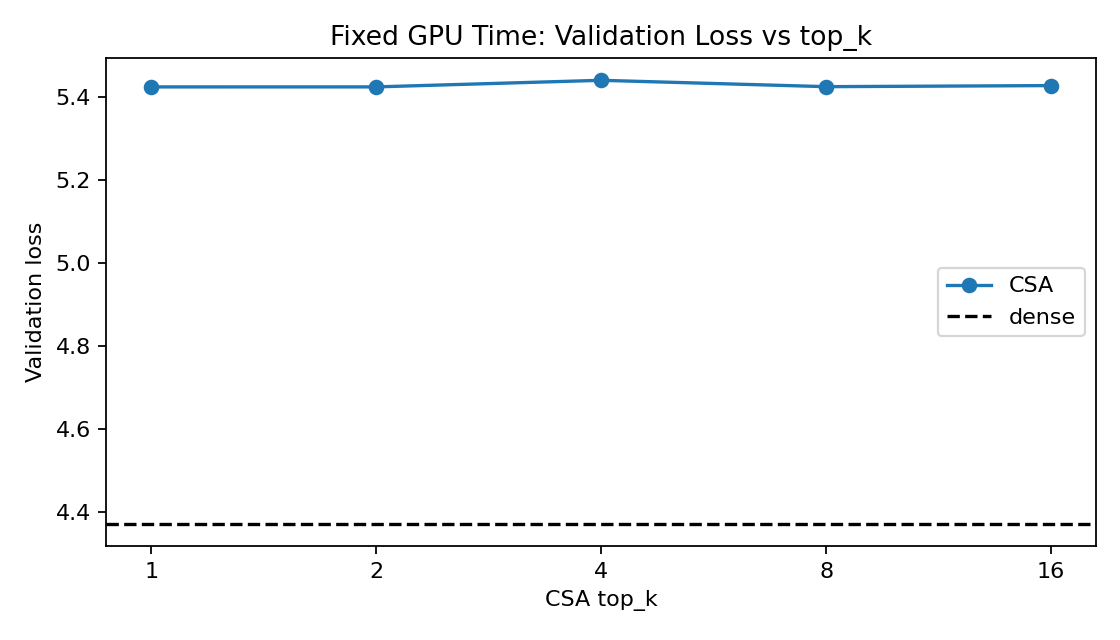
\includegraphics[width=\linewidth]{fixed_time_val_loss_vs_top_k.png}
\caption{Validation loss under equal GPU time.}
\label{fig:val-loss}
\end{subfigure}\hfill
\begin{subfigure}[t]{0.485\textwidth}
\centering
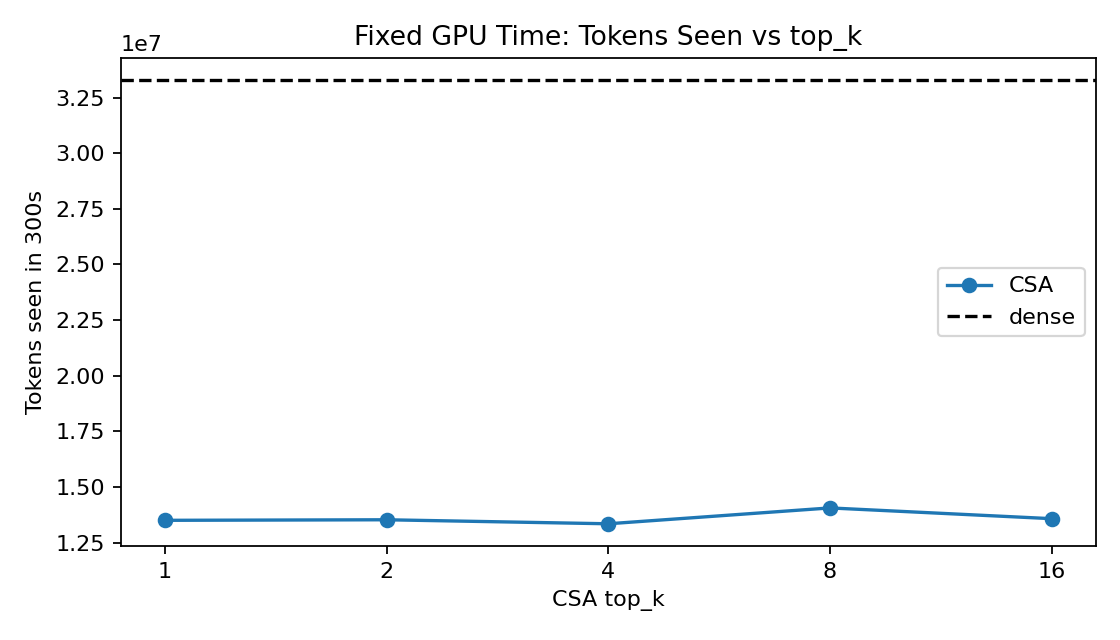
\includegraphics[width=\linewidth]{fixed_time_tokens_seen_vs_top_k.png}
\caption{Tokens processed under equal GPU time.}
\label{fig:tokens}
\end{subfigure}
\caption{The compute-normalized view. Dense sees more data and wins decisively. CSA coverage rises with top-\emph{k}, but the quality curve stays flat in this pilot.}
\label{fig:main}
\end{figure*}

The fixed-token diagnostic, archived alongside the raw results, is less
important. It made CSA look more competitive because every setting saw the same
token budget, but that view is not compute-fair. The compute-normalized view in
Figure~\ref{fig:main} is the headline result.

Increasing top-\emph{k} from 1 to 16 does not produce a recovery curve. CSA
coverage rises from 80 raw-token equivalents to 320, but validation loss stays
clustered around 5.43. Dense reaches 4.37.

\section{Discussion}

The negative result is still useful. It rules out a tempting but too-simple
story:

\begin{quote}
``If we just let CSA read more compressed history, quality will naturally
recover.''
\end{quote}

That did not happen here.

There are several plausible reasons:

\begin{itemize}
\item Plain-PyTorch CSA has overhead that a fused kernel would remove.
\item Dense attention is benefiting from heavily optimized PyTorch paths.
\item The model and training budget may be too small for the top-\emph{k}
knob to matter.
\item The selector or compressor may not yet be learning useful memory.
\end{itemize}

This is why the next experiment is not ``make the model bigger'' but ``make the
question cleaner.'' The simpler follow-up is dense vs local-only vs CSA under
the same GPU-time budget.

\section{Conclusion}

This pilot supports one honest conclusion:

\begin{quote}
Dense attention beats this plain-PyTorch CSA implementation under equal GPU
time.
\end{quote}

That is a negative result for the current implementation, not a verdict on CSA
as a research direction. The paper still does its job because it identifies the
next question instead of hiding the first one.

\begin{thebibliography}{9}
\bibitem{deepseekv4}
DeepSeek-AI.
\newblock {\em DeepSeek-V4: Towards Highly Efficient Million-Token Context Intelligence}.
\newblock 2026.

\bibitem{pytorch}
A.~Paszke et al.
\newblock PyTorch: An Imperative Style, High-Performance Deep Learning Library.
\newblock 2019.
\end{thebibliography}

\end{document}
